%%%%%%%%%%%%%%%%%%%%%%%%%% ch4
\begin{frame}
  \frametitle{主要内容}
  \tableofcontents[hideallsubsections]
\end{frame}

\section{随机过程的统计平均量(from ch2)}

\begin{frame}
\begin{block}{随机过程的均值$\mu_x(t)$: 表示随机过程在$t$时刻状态取值的理论平均值}
	\[\mu_x(t)\mathop{=}^{def}E[x(t)]=\int_{-\infty}^{\infty}xp(x;t)dx \]
	如果$x(t)$是电压或电流,则$\mu_x(t)$可以理解为在$t$时刻的``直流分量''。
\end{block}

\begin{block}{随机过程的均方值$\varphi_x^2(t)$}
	\[\varphi_x^2(t)\mathop{=}^{def}E[x^2(t)]=\int_{-\infty}^{\infty}x^2p(x;t)dx \]
	如果$x(t)$是电压或电流,则$\varphi_x^2(t)$可以理解在$t$时刻它在$1\Omega$电阻上消耗的``平均功率''。
\end{block}
\end{frame}

\begin{frame}
\begin{block}{随机过程的方差/标准偏差$\delta_x^2(t)$}
	\[\sigma_x^2(t)\mathop{=}^{def}E[(x(t)-\mu_x(t))^2]=\int_{-\infty}^{\infty}(x-\mu_x(t))^2p(x;t)dx \]
	方差$\sigma_x^2(t)$表示随机过程在$t$时刻取其值偏离其均值$\mu_x(t)$的离散程度。如果$x(t)$是电压或电流,则$\delta_x^2(t)$可以理解在$t$时刻它在$1\Omega$电阻上消耗的``交流功率''。
\end{block}
\begin{block}{均值$\mu_x(t)$,均方值$\varphi_x^2(t)$,方差$\delta_x^2(t)$之间的关系}
	\[\sigma_x^2(t)=\varphi_x^2(t)-\mu_x^2(t)\]
\end{block}
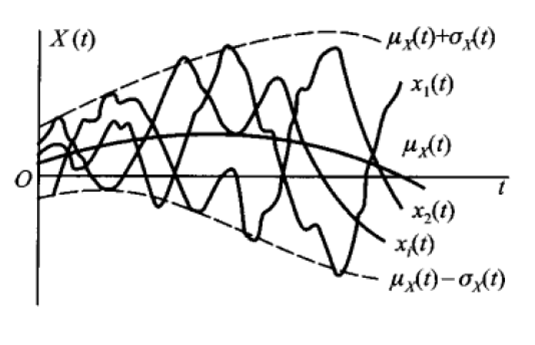
\includegraphics[scale=0.4]{delta}
\end{frame}

\begin{frame}
\begin{block}{随机过程的自相关函数$r_x(t_j,t_k)$}
	\begin{align*}
	r_x(t_j,t_k)&\mathop{=}^{def}E[x(t_j)x(t_k)]\\
	&=\int_{-\infty}^{\infty}	\int_{-\infty}^{\infty}x_jx_kp(x_j,x_k;t_j,t_k)dx_jdx_k
	\end{align*}
\end{block}
随机过程的自相关函数$r_x(t_j,t_k)$可以理解为它的两个随机变量$x(t_j)$与$x(t_k)$之间含有均值时的相关程度的度量。显然
\[r_x(t,t)=\varphi_x^2(t)\]
\end{frame}

\begin{frame}
\begin{block}{随机过程的自协方差函数$c_x(t_j,t_k)$}
	\begin{align*}
	c_x(t_j,t_k)&\mathop{=}^{def}E[((x(t_j)-\mu_x(t_j)(x(t_k)-\mu_x(t_k)]\\
	&=\int_{-\infty}^{\infty}\int_{-\infty}^{\infty}(x_j-\mu_x(t_j))(x_k-\mu_x(t_k))p(x_j,x_k;t_j,t_k)dx_idx_k
	\end{align*}
\end{block}
	随机过程的自协方差函数$c_x(t_j,t_k)$可以理解为它的两个随机变量$x(t_j)$与$x(t_k)$之间的相关程度的度量。它们的自相关系数定义为
\[\rho_x(t_j,t_k)\mathop{=}^{def}\frac{c_x(t_j,t_k)}{\sigma_x(t_j)\sigma_x(t_k)}\]
易证
\[c_x(t_j,t_k)=r_x(t_j,t_k)-\mu_x(t_j)\mu_x(t_k)\]
\[c_x(t,t)=\sigma_x^2(t)\]
\end{frame}

\begin{frame}
\begin{block}{随机过程的互相关函数$r_{xy}(t_j,t_k)$}
	\begin{align*}
	r_{xy}(t_j,t_k) &\mathop{=}^{def}E[x(t_j)y(t_k)]\\
	&=\int_{-\infty}^{\infty}\int_{-\infty}^{\infty}x_jy_kp(x_j,t_j;y_k,t_k)dx_jdy_k
	\end{align*}
	式中, $p(x_j,t_j;y_k,t_k)$是$x(t)$与$y(t)$的二维混合概率密度函数。
\end{block}
\end{frame}

\begin{frame}
\begin{block}{随机过程的互协方差函数$c_{xy}(t_j,t_k)$}
\begin{align*}
c_{xy}(t_j,t_k)&\mathop{=}^{def}E[(x(t_j)-\mu_x(t_j))(y(t_k)-\mu_x(t_k))]\\
&=\int_{-\infty}^{\infty}\int_{-\infty}^{\infty}(x_j-\mu_x(t_j))(y_k-\mu_x(t_k))p(x_j,t_j;x_k,t_k)dx_jdy_k
\end{align*}
\end{block}
随机过程$x(t)$和$y(t)$的互协方差函数$c_{xy}(t_j,t_k)$可以理解为它们各自的随机变量$x(t_j)$与$y(t_k)$之间的相关程度, 实际上表示两个随机过程$x(t)$与$y(t)$之间的相关程度。它们的互相关系数定义为
\[\rho_{xy}(t_j,t_k)\mathop{=}^{def}\frac{c_{xy}(t_j,t_k)}{\sigma_x(t_j)\sigma_x(t_k)}\]
易证
\[c_{xy}(t_j,t_k)=r_{xy}(t_j,t_k)-\mu_x(t_j)\mu_y(t_k)\]
\end{frame}

\section{随机过程的平稳性}

\begin{frame}
\begin{definition}[广义平稳随机过程,简称平稳随机过程]
	随机过程$x(t)$的平均统计量满足
	\begin{enumerate}
		\item $x(t)$的均值是与时间$t$无关的常数,即
		\[E[x(t)]=\mu_x\]
		\item $x(t)$的自相关函数只取决于时间间隔$\tau=t_k-t_j$,而与时间的起始时刻无关,即
		\[E[x(t_j)x(t_k)]=E[x(t_j)x(t_j+\tau)]=r_x(\tau) \]
	\end{enumerate}
\end{definition}
平稳随机过程$x(t)$自相关函数$r_x(t_k-t_j)$仅取决于时间间隔$(t_k-t_j)$,而与时间的起始时刻无关。$E[x(t_j)x(t_k)]=r_x[t_k-t_j]$
\end{frame}

\begin{frame}{平稳随机过程的统计平均量之间的关系}
平稳随机过程x(t)的均值$\mu_x$, 均方值$\varphi_x^2$, 方差$\sigma_x^2$,自相关函数$r_x(\tau)$,自协方差函数$c_x(\tau)$之间的关系
\begin{align*}
&\sigma_x^2=\varphi_x^2-\mu_x^2\\
&r_x(\tau)=r_x(-\tau)\\
&c_x(\tau)=r_x(\tau)-\mu_x^2\\
&c_x(\tau)=c_x(-\tau)\\
&\varphi_x^2=r_x(0)\\
&\sigma_x^2=c_x(0)\\
&r_x(0)\ge|r_x(\tau)|, \tau\ne 0\\
&c_x(0)\ge|c_x(\tau)|, \tau\ne 0
\end{align*}
\end{frame}

\begin{frame}
\begin{definition}[联合平稳随机过程]
	设$x(t)$和$y(t)$分别是两个平稳的随机过程, 如果对于任意的$\Delta t$, 有$r_{xy}(t_j+\Delta t,t_k+\Delta t)=r_{xy}(t_j,t_k)$, 即互相关函数$r_{xy}(t_j,t_k)=r_{xy}(\tau),(\tau=t_k-t_j)$仅与时间间隔$\tau$有关,而与$t_j$和$t_k$无关,则称过程$x(t)$与$y(t)$是联合平稳的随机过程。
\end{definition}
\begin{block}{联合平稳随机过程$x(t)$与$y(t)$的互协方差函数}
	\[c_{xy}(t_j,t_k)=c_{xy}(\tau)=r_{xy}(\tau)-\mu_x\mu_y, \tau=t_k-t_j\]
	互相关系数:
	\[\rho_{xy}(\tau)\mathop{=}^{def}=\frac{c_{xy}(t_j,t_k)}{\sigma_x(t_j)\sigma_y(t_k)}=\frac{c_{xy}(\tau)}{\sigma_x\sigma_y}\]
	\begin{align*}
	r_{xy}(\tau)&=r_{yx}(-\tau)\\
	c_{xy}(\tau)&=c_{yx}(-\tau)
	\end{align*}
\end{block}
\end{frame}

\section{随机过程的正交性、不相关性和统计独立性}

\begin{frame}
\begin{definition}[]
	设$x(t_j)$和$x(t_k)$是随机过程$x(t)$的任意两个不同时刻的随机变量,其均值分别为$\mu_x(t_j)$和$\mu_x(t_k)$, 自相关函数$r_x(t_j,t_k)$, 自协方差函数为$c_x(t_j,t_k)$。如果
	\[r_x(t_j,t_k)=0,j\ne k \]
	则称$x(t)$是相互正交的随机变量过程。如果
	\[c_x(t_j,t_k)=0,j\ne k \]
	则称$x(t)$是互不相关的随机变量过程。等价条件:
	\[c_x(t_j,t_k)=r_x(t_j,t_k)-\mu_x(t_j)\mu_x(t_k), j\ne k \implies r_x(t_j,t_k)=\mu_x(t_j)\mu_x(t_k),j\ne k \]
\end{definition}
\end{frame}

\begin{frame}
\begin{definition}[]
	如果$x(t)$是平稳随机过程,\\
	相互正交:
	\[r_x(\tau)=0,\tau=t_k-t_j\]
	互不相关:
	\[c_x(\tau)=0,\tau=t_k-t_j\]
	互不相关的等价条件
	\[r_x(\tau)=\mu_x^2,\tau=t_k-t_j\]
\end{definition}
\end{frame}

\begin{frame}
\begin{definition}[]
	设$x(t_1),x(t_2),\dots,x(t_N)$是随机过程$x(t)$在不同时刻$t_k(k=1,2,\dots,t_N)$的随机变量, 如果其N维联合概率密度函数对于任意的$N\ge 1$和所有时刻$t_k(k=1,2,\dots,N)$都能够表示成各自一维概率密度函数之积的形式,即
	\begin{align*}
	p(x_1,x_2,\dots,x_N; t_1,t_2,\dots,t_N)\\
	=p(x_1;t_1)p(x_2;t_2)\cdots p(x_N;t_N)
	\end{align*}
	则称$x(t)$是相互统计独立的随机变量过程。
\end{definition}
\end{frame}

\begin{frame}{随机过程的正交性、不相关性和统计独立性}
\begin{enumerate}
	\item 均值$\mu_x(t_j)=0,\mu_x(t_k)=0$则,相互正交$\Leftrightarrow$互不相关
	\item 相互统计独立$\Rightarrow$互不相关
	\item 互不相关$\nRightarrow$相互统计独立。但是若$x(t)$服从联合高斯分布,则互不相关$\Leftrightarrow$相互统计独立
\end{enumerate}
\end{frame}

\section{高斯噪声}

\begin{frame}
\begin{block}{中心极限定理}
	在一般条件下, $N$个相互统计独立的随机变量$n_i$之和$n=\sum\limits_{k=1}^{N}n_k$, 在$N\to\infty$的极限情况下,其概率密度趋于高斯分布,而不管每个变量$n_k$的具体分布如何。
\end{block}
\begin{block}{高斯噪声一维概率密度函数}
	\[p(n_k;t_k)=(\frac{1}{2\pi\sigma_{n_k}^2})^{1/2}\exp[-\frac{(n_k-\mu_{n_k})^2}{2\sigma_{n_k}^2} \]
	其中,$\mu_{n_k}$为$n(t_k)$的均值, $\sigma_{n_k}$为$n(t_k)$的方差。
\end{block}
\end{frame}

\begin{frame}
\begin{block}{高斯噪声N维联合概率密度函数}
	高斯噪声的N维矢量记为
	\[(\mathbf{n;t})=(n(t_1),n(t_2),\cdots,n(t_N))^T \]
	其N维联合概率密度函数为
	\begin{align*}
	p(\mathbf{n;t})&=p(n_1,n_2,\cdots,n_N; t_1,t_2,\cdots,t_N)\\
	&=(\frac{1}{(2\pi)^{N/2}|\mathbf{C}_n|^{1/2}}\exp[-\frac{1}{2}(\mathbf{n-\mu_n})^T\mathbf{C}_n^{-1}(\mathbf{n-\mu_n})]
	\end{align*}
	
	其中,$\mathbf{\mu_{n}}$是高斯随机矢量$(\mathbf{n;t})$的均值矢量,$\mathbf{C}_n$为协方差矩阵。
\end{block}
\begin{block}{不相关性与统计独立性}
	互不相关$\nRightarrow$相互统计独立。但是若$x(t)$服从联合高斯分布,则互不相关$\Leftrightarrow$相互统计独立
\end{block}
\end{frame}

\begin{frame}
\begin{block}{白噪声的功率谱密度}
	\[p_n(\omega)=\frac{N_0}{2}\]
	功率谱密度均匀分布在整个频率轴上
\end{block}
\begin{block}{白噪声的自相关函数}
	\[r_n(\tau)=IFT[\frac{N_0}{2}]=\frac{N_0}{2}\delta(\tau)\]
	白噪声也可定义为均值为零、自相关函数$r_n(\tau)$为$\delta$的噪声随机过程。
\end{block}
\begin{block}{重要特性}
	白噪声在频域上其功率谱密度是均匀分布的,时域上自相关函数$r_n(\tau)$是$\delta$函数。\\
	任意两个不同时刻的随机变量$n(t_j)$与$n(t_k),(\tau=t_j-t_k\ne 0)$是不相关的。
\end{block}
\end{frame}

\begin{frame}
\begin{block}{高斯白噪声}
	时域的随机变量的概率密度函数是高斯分布的,频域的功率谱密度是均匀分布的噪声过程称为高斯白噪声。
	高斯白噪声的重要特性:任意两个或两个以上不同时刻$t_1,t_2,\dots,t_N$的随机变量$n(t_k) (k=1,2,\dots,N)$是互不相关且统计独立的。
\end{block}
\begin{block}{有色噪声的功率谱密度}
	\[P_n(f) =P_0\exp[-\frac{(f-f_0)^2}{2\sigma_f^2}]\]
	均值$f_0$代表频谱的中心频率,方差$\sigma_f^2$反映噪声的谱宽度。$\omega=2\pi f$
\end{block}
\end{frame}

\section{信号分解为正交函数}

\begin{frame}
\begin{block}{矢量正交}
	$\bm{V_x=(V_{x1},V_{x2},V_{x3})}$与$\bm{V_y=(V_{y1},V_{y2},V_{y3})}$,正交的定义: 其\textbf{内积}为0。即
	\[\bm{V_xV_y}=\sum_{i=1}^{3}v_{xi}v_{yi}=0 \]
\end{block}
\begin{block}{正交矢量集}
	由两两正交的矢量组成的矢量集合称为正交矢量集。
\end{block}
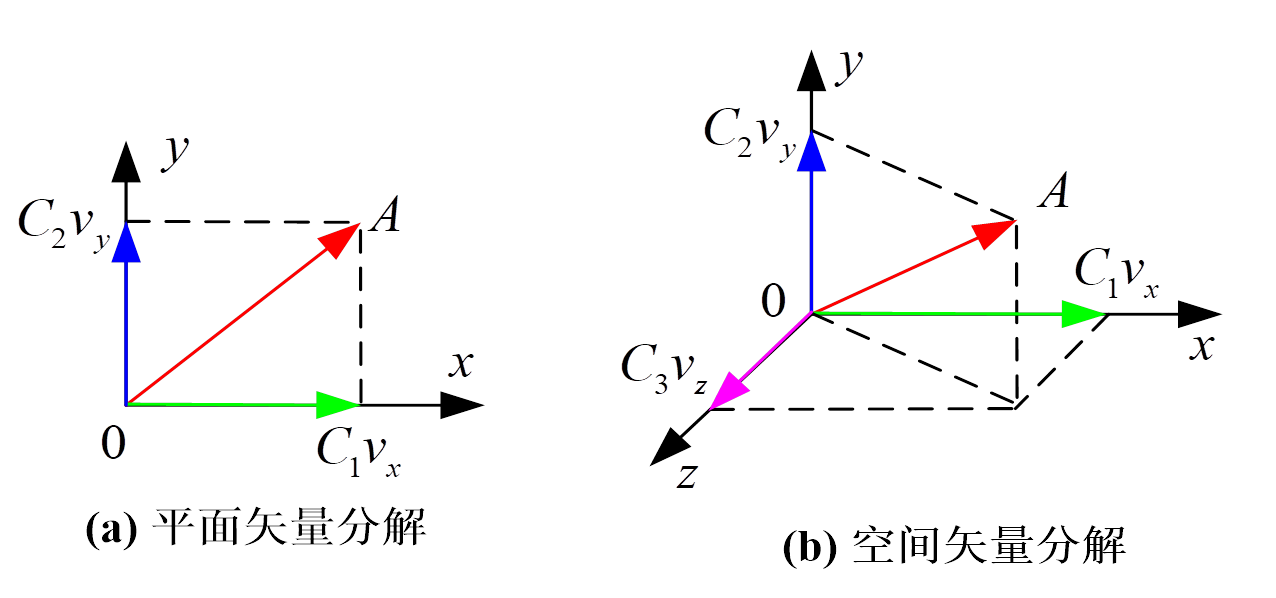
\includegraphics[scale=0.3]{vector}
\end{frame}

\begin{frame}
\begin{example}
	如三维空间中,以矢量$\bm{v_x}=(2,0,0),\bm{v_y}=(0,2,0),\bm{v_z}=(0,0,2)$所组成的集合就是一个\textbf{正交矢量集}。\\
	对于一个三维空间的矢量$\bm{A}=(2,5,8)$,可以用一个三维正交矢量集$\{v_x,v_y,v_z\}$分量的线性组合表示。即
	\[\bm{A=v_x+2.5v_y+4v_z} \]
\end{example}
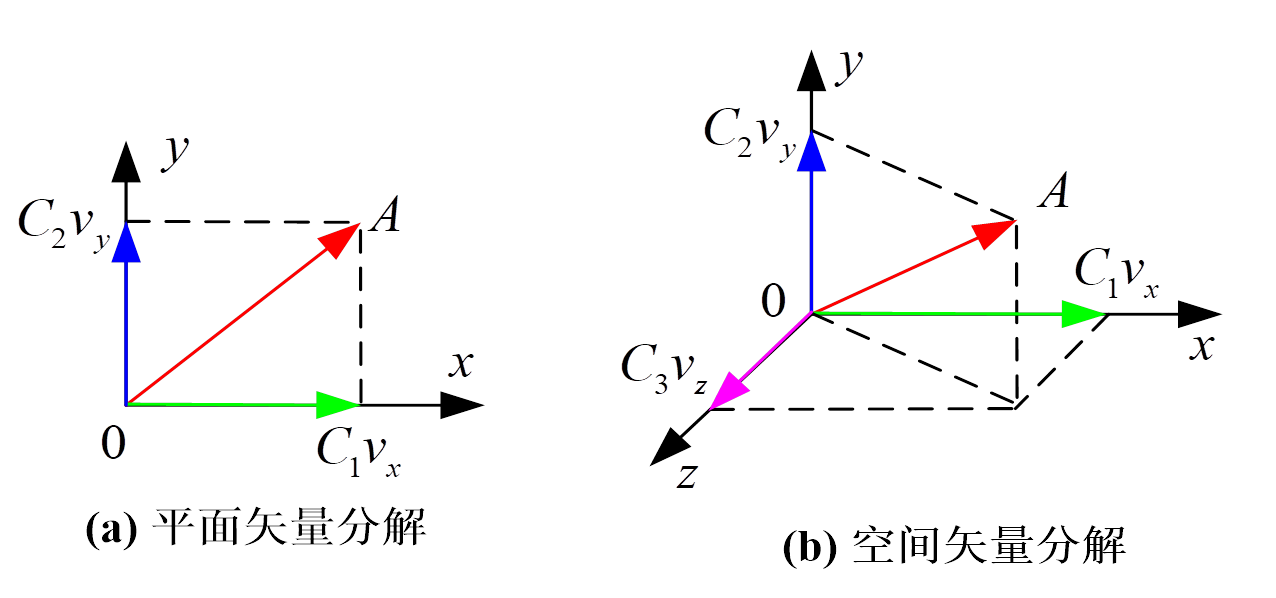
\includegraphics[scale=0.3]{vector}
\end{frame}

\begin{frame}
矢量空间正交分解的概念可推广到信号空间:在信号空间找到若干个\textbf{相互正交}的信号作为基本信号,使得信号空间中\textbf{任意信号均可表示成它们的线性组合}。 

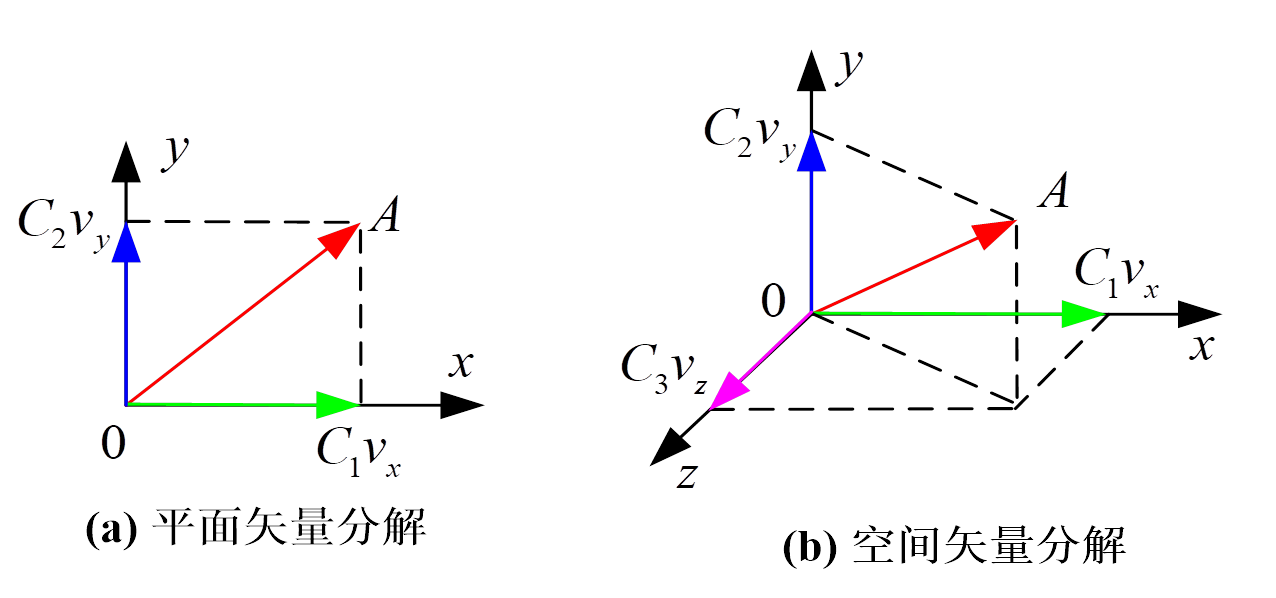
\includegraphics[scale=0.3]{vector}
\end{frame}

\begin{frame}{完备正交函数集}
三角函数集$\{1,\cos(n\omega t),\sin(n\omega t),\dots\},n=1,2,\dots$。就是在区间$(t_0,t_0,T),T=2\pi/\omega$上的完备正交函数集。
\begin{example}[傅里叶级数的三角形式]
	$f(t)=\frac{a_0}{2}+\sum\limits_{n=1}^{\infty}a_n\cos(n\omega t)+\sum\limits_{n=1}^{\infty}b_n\sin(n\omega t)$\\
	傅里叶系数: $a_n=\frac{2}{T}\int_{-\frac{T}{2}}^{\frac{T}{2}}f(t)\cos(n\omega t)dt$,\quad $b_n=\frac{2}{T}\int_{-\frac{T}{2}}^{\frac{T}{2}}f(t)\sin(n\omega t)dt$
\end{example}
\end{frame}

\begin{frame}{正交级数展开}
\begin{table}[htbp!]
\small
%\centering
\caption{正交级数展开}
\begin{tabular}{|c|c|c|c|}
	%\begin{tabular}{|p{1cm}|p{2cm}|p{2cm}|p{2cm}|}
	\hline 
	& 二维矢量 & 信号$f(t)$傅里叶展开 & 信号$x(t)$正交级数 \\ 
	\hline 
	正交集 & $\{\bm{v_x,v_y}\}$ & $\{1,\cos(n\omega t),\sin(n\omega t)\}$ & $\{f_1(t),f_2(t),\dots,f_k(t)\}$ \\ 
	\hline 
	展开系数 & $C_k=$矢量$\bm{A}$在 &
	 $a_n=\frac{2}{T}\int_{-\frac{T}{2}}^{\frac{T}{2}}f(t)\cos(n\omega t)dt$ & $x_k=\int_{0}^{T}f_k(t)x(t)dt$ \\  
	(正交投影)& 第$k$个坐标的投影&$b_n=\frac{2}{T}\int_{-\frac{T}{2}}^{\frac{T}{2}}f(t)\sin(n\omega t)dt$& $$\\ 
	\hline 
	线性表示 & $\bm{A=C_1v_x+C_2v_y}$ & $f(t)=\frac{a_0}{2}+\sum\limits_{n=1}^{\infty}a_n\cos(n\omega t)$ & $x(t)=\lim\limits_{N\to\infty}\sum\limits_{k=1}^{N}x_kf_k(t)$ \\ 
	& & $+\sum\limits_{n=1}^{\infty}b_n\sin(n\omega t)$ &  \\ 
	\hline 
\end{tabular} 
\end{table}

%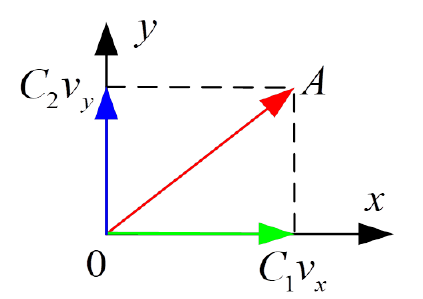
\includegraphics[scale=0.3]{vector1}
\end{frame}

\begin{frame}{确知信号的正交级数展开}
	$s(t)$是定义在(0,T)时间内的确知信号
\end{frame}

\begin{frame}{随机过程的正交级数展开}
随机过程$x(t)$展开的均方误差等于0,\\ 或者说$\lim\limits_{N\to\infty}\sum\limits_{k=1}^{N}x_kf_k(t)$均方收敛于$x(t)$
\end{frame}

\begin{frame}{随机过程的正交级数展开}
\begin{block}{Notes}
随机过程: $x(t)=\lim\limits_{N\to\infty}^N\sum\limits_{k=1}^Nx_kf_k(t)$\\
展开系数: $x_k=\int_{0}^{T}x(t)f_k(t)dt, k=1,2,\dots$\\
随机过程$x(t)$可以由上式求得的展开系数$x_k$来恢复,就是说$x(t)$完全由展开系数$x_k$确定。注意,这里对随机过程$x(t)$进行正交级数展开所用的正交函数集$\{f_k(t)\}$并没有提出特别的要求,所以\textbf{展开系数$x_k(k=1,2,\dots)$之间可能是相关的随机变量}。\\
\end{block}
\begin{block}{问题}
	如何根据噪声干扰的特性,正确选择随机过程展开的正交函数集$\{f_k\}$,以使展开系数$x_k$之间是互不相关的随机变量。
\end{block}
\end{frame}

\begin{frame}{$x_k,s_k,n_k$之间的关系}
\begin{block}{$x_k,s_k,n_k$之间的关系}
	\[x(t)=s(t)+n(t); \quad x_k=s_k+n_k \]
	随机变量$x(t)$展开系数$x_k$=确知信号$s(t)$展开系数$s_k$+噪声$n(t)$展开系数$n_k$
\end{block}
\begin{align*}
x_k&=\int_{0}^{T}f_k(t)x(t)dt\\
&=\int_{0}^{T}f_k(t)(s(t)+n(t))dt\\
&=\int_{0}^{T}f_k(t)s(t)dt+\int_{0}^{T}f_k(t)n(t))dt\\
&=s_k+n_k
\end{align*}
\end{frame}

\begin{frame}{展开系数级数展开-准备公式}
\begin{itemize}
	\item 随机过程: $x(t)=s(t)+n(t)$
	\item $\{f_k(t)\}$是一组正交函数集, $k=1,2,\dots$
	\item 随机过程$x(t)的$正交展开系数$x_k$是一个随机变量: $x_k=\int_{0}^{T}x(t)f_k(t)dt$
	\item 确知信号$s(t)$正交展开系数$s_k$是一个确定的量: $s_k=\int_{0}^{T}s(t)f_k(t)dt$
	\item 确知信号$s(t)$的展开系数$s_k$为确定的量,其均值就是本身: $E(s_k)=E\left[\int_{0}^{T}s(t)f_k(t)dt\right]=\int_{0}^{T}E[s(t)]f_k(t)dt=\int_{0}^{T}s(t)f_k(t)dt=s_k$
	\item 噪声$n(t)$是一个零均值的平稳随机过程:
	\begin{itemize}
		\item[-] $E[n(t)]=0$
		\item[-]  $n(t)$的自相关函数只取决于时间间隔$(t_k-t_j)$,而与时间的起始时刻无关,$E[n(t_j)n(t_k)]=r_n(t_k-t_j)$
	\end{itemize}
\end{itemize}
\end{frame}

\begin{frame}{展开系数$x_k$均值(推导一)}
\begin{align*}
E[x_k]&=E\left[\int_{0}^{T}f_k(t)x(t)dt\right]=E\left[\int_{0}^{T}f_k(t)(s(t)+n(t))dt\right]\\
&=E\left[\int_{0}^{T}f_k(t)s(t)dt+\int_{0}^{T}f_k(t)n(t))dt\right]\\
&=E[s_k+n_k]\\
&=E[s_k]+E[n_k]\qquad (\text{by }E[n(t)]=0\implies E[n_k]=0)\\
&= E[s_k] = s_k\qquad \text{(确知信号的展开系数为确定的量,其均值就是本身)}
\end{align*}
\end{frame}

\begin{frame}{展开系数$x_k$均值(推导二),课件采用}
\begin{align*}
E[x_k]&=E\left[\int_{0}^{T}f_k(t)x(t)dt\right]=E\left[\int_{0}^{T}f_k(t)(s(t)+n(t))dt\right]\\
&=E\left[\int_{0}^{T}f_k(t)s(t)dt+\int_{0}^{T}f_k(t)n(t))dt\right]\\
&=E\left[\int_{0}^{T}f_k(t)s(t)dt\right]+E\left[\int_{0}^{T}f_k(t)n(t))dt\right]\\
&=E\left[\int_{0}^{T}f_k(t)s(t)dt\right]+\int_{0}^{T}f_k(t)E[n(t))]dt \qquad  (\text{by }E[n(t)]=0)\\
&=E\left[\int_{0}^{T}f_k(t)s(t)dt\right]\\
&= E[s_k] = s_k\qquad \text{  (确知信号的展开系数为确定的量,其均值就是本身)}
\end{align*}
\end{frame}

\begin{frame}{展开系数$x_j$与$x_k$协方差,在t时刻两个随机变量减去各自的均值后的乘积}
\begin{align*}
&E[(x_j-E(x_j))(x_k-E(x_k))]=E[(x_j-s_j)(x_k-s_k)]\\
&=E\left[\left(\int_{0}^{T}f_j(t)x(t)dt-s_j\right)\left(\int_{0}^{T}f_k(t)x(t)dt-s_k\right)\right]\\
&=E\left[\left(\int_{0}^{T}f_j(t)(s(t)+n(t))dt-s_j\right)\left(\int_{0}^{T}f_k(t)(s(t)+n(t))dt-s_k\right)\right]\\
&=E\left[\left(\int_{0}^{T}f_j(t)n(t)dt\right)\left(\int_{0}^{T}f_k(t)n(t)dt\right)\right]=E\left[\left(\int_{0}^{T}f_j(t)n(t)dt\right)\left(\int_{0}^{T}f_k(u)n(t)du\right)\right]\\
&=E\left[\int_{0}^{T}f_j(t)\left[\int_{0}^{T}n(t)n(u)f_k(u)du\right]dt\right]=\int_{0}^{T}f_j(t)\left[\int_{0}^{T}E[n(t)n(u)]f_k(u)du\right]dt\\
&=\int_{0}^{T}f_j(t)\left[\int_{0}^{T}r_n(t-u)f_k(u)du\right]dt\quad (\text{by }E[n(t_j)n(t_k)]=r_n(t_k-t_j))
\end{align*}
\end{frame}

\begin{frame}{随机过程的卡亨南-洛维展开}
希望$x(t)$各展开系数$x_j$与$x_k$的协方差满足:
\[E[(x_j-E(x_j))(x_k-E(x_k))]=E[(x_j-s_j)(x_k-s_k)]=\lambda_k\delta_{jk} \]
式中$\delta_{jk}=
\begin{cases}
1, & (j=k)\\
0, & (j\ne k)
\end{cases}$, $\lambda_k$是展开系数$x_k$的方差, $k=1,2,\dots$\\
这样,当$j\ne k$时, $E[(x_j-s_j)(x_k-s_k)]=0$,即展开式的各展开系数之间互不相关; 当$j=k$时, $E[(x_j-s_j)(x_k-s_k)]=\lambda_k$, 是展开系数$x_k$的方差。
\end{frame}

\begin{frame}{随机过程的卡亨南-洛维展开}
展开系数$x_j$与$x_k$协方差:
\[E[(x_j-s_j)(x_k-s_k)]=\int_{0}^{T}f_j(t)\left[\int_{0}^{T}r_n(t-u)f_k(u)du\right]dt \]
其中, $x(t)=s(t)+n(t)(0\le t\le T),r_n(t-u)=E[n(t)n(u)]$是零均值平稳噪声过程$n(t)$的自相关函数。

为保证$E[(x_j-s_j)(x_k-s_k)]=\lambda_k\delta_{jk}$
\[\int_{0}^{T}r_n(t-u)f_k(u)du=\lambda_kf_k(t), 0\le t\le T \]
该式是齐次积分方程。该方程的解$f_k(t)$就是正交函数集$\{f_k(t) \}$的第$k$个坐标函数。

$E[(x_j-s_j)(x_k-s_k)]=\lambda_k\int_{0}^{T}f_j(t)f_k(t)dt=\lambda_k\delta_{jk}\implies f_j(t)$与$f_k(t)$正交。
\end{frame}

\begin{frame}{白噪声条件下正交函数集的任意性(1)}
假设接收信号为$x(t)=s(t)+n(t)$, $n(t)$是零均值,功率谱密度为$P_n(\omega)=N_0/2$的白噪声,其自相关函数为: $r_n(t-u)=\frac{N_0}{2}\delta(t-u)$,(说明噪声自相关函数在$t=u$时不为0,其他时刻都为0,自相关性最强)\\
对于任意招教函数集$\{f_k(t)\}$,展开系数$x_j$与$x_k$协方差:
\begin{align*}
E[(x_j-s_j)(x_k-s_k)]&=\int_{0}^{T}f_j(t)\left[\int_{0}^{T}r_n(t-u)f_k(u)du\right]dt\\
&=\frac{N_0}{2}\int_{0}^{T}f_j(t)\left[\int_{0}^{T}\delta(t-u)f_k(u)du\right]dt\\
&=\frac{N_0}{2}\int_{0}^{T}f_j(t)f_k(t)dt=\frac{N_0}{2}\delta_{jk}
\end{align*}
式中$\delta_{jk}=
\begin{cases}
1, & (j=k)\\
0, & (j\ne k) 
\end{cases},\quad
\delta(t-u)=
\begin{cases}
	1, & (t=u)\\
	0, & (t\ne u) 
\end{cases}
$
\end{frame}

\begin{frame}{白噪声条件下正交函数集的任意性(1)}
假设接收信号为$x(t)=s(t)+n(t)$, $n(t)$是零均值,功率谱密度为$P_n(\omega)=N_0/2$的白噪声,其自相关函数为: 
\[r_n(t-u)=\frac{N_0}{2}\delta(t-u)\]
对于任意招教函数集$\{f_k(t)\}$,展开系数$x_j$与$x_k$协方差:
\begin{align*}
E[(x_j-s_j)(x_k-s_k)]=\int_{0}^{T}f_j(t)\left[\int_{0}^{T}r_n(t-u)f_k(u)du\right]dt=\frac{N_0}{2}\delta_{jk}
\end{align*}
\begin{block}{重要结论}
	当$j\ne k$时,展开系数$x_j$与$x_k$协方差=0。这说明,在$n(t)$是白噪声的条件下,取任意正交函数集$\{f_k(t)\}$对平稳随机过程$x(t)$进行展开,其展开系数$x_k(k=1,2,\dots)$之间都是互不相关的。
	这就是白噪声条件下正交函数集的任意性。
\end{block}
\end{frame}

\begin{frame}{白噪声条件下正交函数集的任意性(2)}
\[r_n(t-u)=\frac{N_0}{2}\delta(t-u) \]
展开系数$x_j$与$x_k$协方差:
\begin{align*}
E[(x_j-s_j)(x_k-s_k)]&=\int_{0}^{T}f_j(t)\left[\int_{0}^{T}r_n(t-u)f_k(u)du\right]dt\\
&=\frac{N_0}{2}\int_{0}^{T}f_j(t)\left[\int_{0}^{T}\delta(t-u)f_k(u)du\right]dt\\
&=\frac{N_0}{2}\int_{0}^{T}f_j(t)f_k(t)dt=\frac{N_0}{2}\delta_{jk}
\end{align*}
\end{frame}

\begin{frame}{二元信号波形检测}
\tikzstyle{int}=[draw, fill=blue!20, minimum size=2em]
\begin{tikzpicture}[node distance=3.5cm,auto,>=latex']
\node [int] (a) {$x(t)$};
\node [int] (b) [right of=a] {$x_k$};
\node [int] (c) [right of=b] {$x_N$};
\node [int] (d) [below of=c] {$\frac{p(x_N|H_1)}{p(x_N|H_0)}\mathop{\gtrless}_{H_0}^{H_1}\eta$};
\node [int] (e) [left of=d] {$l(x)\mathop{\gtrless}_{H_0}^{H_1}\gamma$};
\path[->] (a) edge node {$\{f_k(t)\}$正交展开} (b);
\path[->] (b) edge node {前N项$x_k$构成$x_N$} (c);
\path[->] (c) edge [swap] node {贝叶斯检测} (d);
\path[->] (d) edge [swap] node {$N\to\infty$} (e);
\end{tikzpicture}
\end{frame}

\begin{frame}{简单二元信号波形检测}
\begin{columns}
	\column{0.4\textwidth}
	$H_0: x(t)=n(t)$\\
	$H_1: x(t)=s(t)+n(t)$\\
	$x(t)=\lim\limits_{N\to\infty}^N\sum\limits_{k=1}^Nx_kf_k(t)$\\
	$x_k=\int_{0}^{T}x(t)f_k(t)dt, k=1,2,\dots$\\
	$s_k=\int_{0}^{T}s(t)f_k(t)dt, k=1,2,\dots$\\
	$n_k=\int_{0}^{T}n(t)f_k(t)dt, k=1,2,\dots$\\
	$H_0: x_k=n_k,k=1,2,\dots$\\
	$H_1: x_k=s_k+n_k,k=1,2,\dots$
	\column{0.6\textwidth}
	\begin{itemize}
		\item 信号s(t)是确知信号,n(t)是均值为0,功率谱密度为$P_n(\omega)=N_0/2$的高斯白噪声;
		\item 无论在假设$H_1$下还是在假设$H_2$下,接收信号的$x(t)$都是高斯随机过程;
		\item 展开系数$x_k$是高斯随机过程的积分结果,因而$x_k$是高斯随机变量;
		\item 展开系数$x_k$之间是互不相关的,也是相互统计独立的;
		\item 高斯随机变量由均值和方差决定。由此求出两个假设下的概率密度函数$p(x_k|H_j),k=1,2,\dots;j=0,1$。
	\end{itemize}
\end{columns}
\end{frame}

\begin{frame}{简单二元信号波形检测$H_0$}
$n(t)$是高斯白噪声$\implies E[n(t)n(u)]=r_n(t-u) =\frac{N_0}{2}\delta(t-u)=\frac{N_0}{2},(\delta(t-u)=1,t=u)$ \\
$f_k(t)$是一组正交函数集$\implies\int_{0}^{T}f_j(t)f_k(t)dt=1,(j=k)$
\begin{align*}
Var[x_k|H_0]&=E[n_k^2]=E\left[\int_{0}^{T}n(t)f_k(t)dt\int_{0}^{T}n(u)f_k(u)du\right]\\
&=\int_{0}^{T}f_k(t)\left\{\int_{0}^{T}E[n(t)n(u)]f_k(u)du\right\}dt\\
&=\int_{0}^{T}f_k(t)\left[\int_{0}^{T}\frac{N_0}{2}\delta(t-u)f_k(u)du\right]dt\\
&=\int_{0}^{T}f_k(t)\frac{N_0}{2}f_k(t)dt\\
&=\frac{N_0}{2}
\end{align*}
\end{frame}

\begin{frame}{简单二元信号波形检测$H_1$}
$x_k=\int_{0}^{T}x(t)dt=\int_{0}^{T}[s(t)+n(t)]dt=\int_{0}^{T}s(t)dt+\int_{0}^{T}n(t)dt=s_k+n_k$\\
$x_k=s_k+n_k$
\begin{align*}
E[x_k|H_1]&=E[s_k+n_k]&\text{by }x_k=s_k+n_k \\
&=E(s_k)+E(n_k)&\text{by }E(n_k)=0 \\
&=E(s_k)=s_k&\text{(确知信号展开系数为确定量,其均值就是本身)}\\
Var[x_k|H_1]&=E[(x_k-E[x_k])^2]&\text{by }x_k=s_k+n_k,E[x_k]=s_k\\
&=E[(s_k+n_k-s_k)^2]&\\
&=E[n_k^2]=\frac{N_0}{2}&
\end{align*}
或: $E[x_k|H_1]=E\left[\int_{0}^{T}x(t)f_k(t)dt\right]=E\left[\int_{0}^{T}(s(t)+n(t))f_k(t)dt\right]$\\
$=E\left[\int_{0}^{T}s(t)dt\right]+\int_{0}^{t}E[n(t)])f_k(t)dt=E\left[\int_{0}^{T}s(t)dt\right]=E[s_k]=s_k$
\end{frame}

\begin{frame}{简单二元信号波形检测-判决式预备公式}
\[\ln\lambda(\bm{x}_N)=\frac{p(\bm{x}_N|H_1)}{p(\bm{x}_N|H_0)}=\frac{2}{N_0}\sum\limits_{k=1}^{N}x_ks_k-\frac{1}{N_0}\sum\limits_{k=1}^{N}s_k^2\mathop{\gtrless}_{H_0}^{H_1}\ln\eta \]
\begin{align*}
&x(t)=\lim\limits_{N\to\infty}\sum\limits_{k=1}^Nx_kf_k(t)\\
&x_k=\int_{0}^{T}x(t)f_k(t)dt, k=1,2,\dots\\
&s(t)=\lim\limits_{N\to\infty}\sum\limits_{k=1}^Ns_kf_k(t)\\
&s_k=\int_{0}^{T}s(t)f_k(t)dt, k=1,2,\dots\\
&E_s=\int_{0}^{T}s^2(t)dt
\end{align*}
\end{frame}

\begin{frame}{简单二元信号波形检测-判决式推导(1)}
\begin{align*}
\lim\limits_{N\to\infty}\sum\limits_{k=1}^{N}x_ks_k&=\left[\lim\limits_{N\to\infty}\sum\limits_{k=1}^{N}x_k\right]s_k\\
&=\left[\lim\limits_{N\to\infty}\sum\limits_{k=1}^{N}x_k\right]\int_{0}^{T}s(t)f_k(t)dt\\
&=\int_{0}^{T}s(t)\left[\lim\limits_{N\to\infty}\sum\limits_{k=1}^{N}x_kf_k(t)\right]dt\\
&=\int_{0}^{T}s(t)x(t)dt
\end{align*}
\end{frame}

\begin{frame}{简单二元信号波形检测-判决式推导(2)}
\begin{align*}
\lim\limits_{N\to\infty}\sum\limits_{k=1}^{N}s_k^2&=\left[\lim\limits_{N\to\infty}\sum\limits_{k=1}^{N}s_k\right]s_k\\
&=\left[\lim\limits_{N\to\infty}\sum\limits_{k=1}^{N}s_k\right]\int_{0}^{T}s(t)f_k(t)dt\\
&=\int_{0}^{T}s(t)\left[\lim\limits_{N\to\infty}\sum\limits_{k=1}^{N}s_kf_k(t)\right]dt\\
&=\int_{0}^{T}s(t)s(t)dt=\int_{0}^{T}s^2(t)dt=E_s
\end{align*}
\end{frame}

\begin{frame}{简单二元信号波形检测-检测性能(1)}
\textbf{判决表达式:}
\[l[x(t)]\mathop{=}^{def}\int_{0}^{T}x(t)s(t)dt\mathop{\gtrless}_{H_0}^{H_1}\frac{N_0}{2}\ln\eta+\frac{E_s}{2}\mathop{=}^{def}\gamma \]
检验统计量$l[x(t)]$无论在假设$H_0$下,还是在假设$H_1$下,都是由高斯随机过程$x(t)s(t)(0\le t\le T)$经积分得到的,所以\bm{$l[x(t)]$}\textbf{是高斯随机变量}。
\begin{enumerate}
	\item 求出检验统计量$l[x(t)]$在两个假设下的均值$E(l|H_j)$和方差$Var(l|H_j),j=0,1$;
	\item 求各种判决概率$P(H_i|H_j),i,j=0,1$;\\
	简单二元信号检测与雷达信号检测相对应:$P(H_1|H_0)\mathop{=}\limits^{def}P_F$(称为虚警概率),$P(H_1|H_1)\mathop{=}\limits^{def}P_D$(称为检测概率)
	\item 计算检测性能。
\end{enumerate}
\end{frame}

\begin{frame}{简单二元信号波形检测-检测性能(2)}
\begin{enumerate}[1]
	\item 定义统计量:$l\mathop{=}\limits^{def}\int_{0}^{T}x(t)s(t)dt$
	\item 假设$H_0,H_1$下检验统计量$l[x(t)]$的均值和方差分别为\\
	$E[l|H_0]=E\left[\int_{0}^{T}x(t)s(t)dt|H_0\right]=E\left[\int_{0}^{T}n(t)s(t)dt\right]=0$\\ 
	$Var[l|H_0]=E[((l|H_0)-E(l|H_0))^2]=\frac{N_0}{2}E_s$\\
	$E[l|H_1]=E\left[\int_{0}^{T}x(t)s(t)dt|H_1\right]=E\left[\int_{0}^{T}(s(t)+n(t))s(t)dt\right]=E_s$\\
	$Var[l|H_1]=E[((l|H_1)-E(l|H_1))^2]=\frac{N_0}{2}E_s$\\
	\item 假设$H_0,H_1$下服从高斯分布的检验统计量$l[x(t)]$的概率密度函数分别为\\
\[p(l|H_0)=\left(\frac{1}{\pi N_0E_s}\right)^{1/2}\exp\left(-\frac{l^2}{N_0E_s}\right)\]
	\[p(l|H_1)=\left(\frac{1}{\pi N_0E_s}\right)^{1/2}\exp\left(-\frac{(l-E_s)^2}{N_0E_s}\right)\]
\end{enumerate}
\end{frame}
\begin{frame}{简单二元信号波形检测-检测性能(3)}
\begin{enumerate}
	\setcounter{enumi}{3} 
	\item 求各种判决概率$P(H_i|H_j),i,j=0,1$\\
	虚警概率:$P(H_1|H_0)\mathop{=}\limits^{def}P_F=Q\left[\frac{\ln\eta}{d}+\frac{d}{2}\right]$\\ 检测概率:$P(H_1|H_1)\mathop{=}\limits^{def}P_D=Q\left[\frac{\ln\eta}{d}-\frac{d}{2}\right]$\\
	$P(H_0|H_1)=1-P(H_1|H_1)=1-Q\left[\frac{\ln\eta}{d}-\frac{d}{2}\right]$\\
	$P(H_0|H_0)=1-P(H_1|H_0)=1-Q\left[\frac{\ln\eta}{d}+\frac{d}{2}\right]$\\
	$d^2\mathop{=}\limits^{def}\frac{(E(l|H_1)-E(l|H_0))^2}{Var(l|H_0)}=\frac{2E_s}{N_0}$ \qquad 偏移系数$d^2$表示功率信噪比\\
\end{enumerate}
\begin{block}{结论}
	对简单二元信号来讲,只要保持确知信号$s(t)$的能量不变,信号波形可以任意设计,检测性能不发生变化。
\end{block}
\end{frame}

\begin{frame}{计算$E[l|H_0]$}
\begin{align*}
E[l|H_0]&=E\left[\int_{0}^{T}x(t)s(t)dt|H_0\right] &\text{by }H_0: x(t)=n(t)\\
&=E\left[\int_{0}^{T}n(t)s(t)dt\right]&\\
&=\int_{0}^{T}E[n(t)]s(t)dt=0 &\text{by }E[n(t)]=0
\end{align*}
\end{frame}

\begin{frame}{计算$Var[l|H_0]$}
$H_0:x(t)=n(t), E(l|H_0)=0,E_s=\int_{0}^{T}s^2(t)dt$\\
$E[n(t)n(u)=r_n(t-u)=\frac{N_0}{2}\delta(t-u)=\frac{N_0}{2},(t=u,\delta(t-u)=1)$
\begin{align*}
Var[l|H_0]&=E[((l|H_0)-E(l|H_0))^2]=E[(l|H_0)^2]=E\left[\left(\int_{0}^{T}x(t)s(t)dt\right)^2\right]\\
&=E\left[\int_{0}^{T}n(t)s(t)dt\int_{0}^{T}n(t)s(t)dt\right]=E\left[\int_{0}^{T}n(t)s(t)dt\int_{0}^{T}n(u)s(u)du\right]\\
&=\int_{0}^{T}s(t)\left\{\int_{0}^{T}E[n(u)n(t)]s(u)du\right\}dt=\int_{0}^{T}s(t)\left[\int_{0}^{T}\frac{N_0}{2}\delta(t-u)s(u)du\right]dt\\
&=\frac{N_0}{2}\int_{0}^{T}s(t)\left(\int_{0}^{T}s(u)du\right)dt=\frac{N_0}{2}\int_{0}^{T}s^2(t)dt\\
&=\frac{N_0}{2}E_s
\end{align*}
\end{frame}

\begin{frame}{计算$p(l|H_0)$}
$E[l|H_0]=0,Var[l|H_0]=\frac{N_0}{2}E_s$
\begin{align*}
p(l|H_0)&=\left(\frac{1}{2\pi Var[l|H_0]}\right)^{1/2}\exp\left(-\frac{(l-E[l|H_0])^2}{2Var[l|H_0]}\right)\\
&=\frac{1}{\sqrt{\pi N_0E_s}}\exp\left(-\frac{l^2}{N_0E_s}\right)
\end{align*}
\end{frame}

\begin{frame}{计算$E[l|H_1]$}
\begin{align*}
E[l|H_1]&=E\left[\int_{0}^{T}x(t)s(t)dt|H_1\right] &\text{by }H_1: x(t)=s(t)+n(t)\\
&=E\left[\int_{0}^{T}(s(t)+n(t))s(t)dt\right]&\\
&=E\left[\int_{0}^{T}s^2(t)dt\right]+\int_{0}^{T}E[n(t)]s(t)dt& \text{by } E[n(t)]=0 \\
&=E\left[\int_{0}^{T}s^2(t)dt\right]& \text{by } E_s=\int_{0}^{T}s^2(t)dt 
&=E_s
\end{align*}
\end{frame}

\begin{frame}{计算$Var[l|H_1]$}
$H_1:x(t)=s(t)+n(t), E(l|H_1)=E_s,E_s=\int_{0}^{T}s^2(t)dt$\\
$E[n(t)n(u)=r_n(t-u)=\frac{N_0}{2}\delta(t-u)=\frac{N_0}{2},(t=u,\delta(t-u)=1)$
\begin{align*}
Var[l|H_1]&=E[((l|H_1)-E(l|H_1))^2]=E\left[\left(\int_{0}^{T}(s(t)+n(t))s(t)dt-E_s\right)^2\right]\\
&=E\left[\left(\int_{0}^{T}(s^2(t)dt+\int_{0}^{T}n(t)s(t)dt-E_s\right)^2\right]=E\left[\left(\int_{0}^{T}n(t)s(t)dt\right)^2\right]\\
&=E\left[\int_{0}^{T}n(t)s(t)dt\int_{0}^{T}n(t)s(t)dt\right]=E\left[\int_{0}^{T}n(t)s(t)dt\int_{0}^{T}n(u)s(u)du\right]\\
&=\int_{0}^{T}s(t)\left\{\int_{0}^{T}E[n(u)n(t)]s(u)du\right\}dt=\int_{0}^{T}s(t)\left[\int_{0}^{T}\frac{N_0}{2}\delta(t-u)s(u)du\right]dt\\
&=\frac{N_0}{2}\int_{0}^{T}s(t)\left(\int_{0}^{T}s(u)du\right)dt=\frac{N_0}{2}\int_{0}^{T}s^2(t)dt=\frac{N_0}{2}E_s
\end{align*}
\end{frame}

\begin{frame}{计算$p(l|H_1)$}
$E[l|H_1]=E_s,Var[l|H_1]=\frac{N_0}{2}E_s$
\begin{align*}
p(l|H_1)&=\left(\frac{1}{2\pi Var[l|H_1]}\right)^{1/2}\exp\left(-\frac{(l-E[l|H_1])^2}{2Var[l|H_1]}\right)\\
&=\frac{1}{\sqrt{\pi N_0E_s}}\exp\left(-\frac{(l-E_s)^2}{N_0E_s}\right)
\end{align*}
\end{frame}

\begin{frame}{计算$P(H_1|H_0)$}
\begin{align*}
P(H_1|H_0)&\mathop{=}^{def}P_F=\int_{\gamma}^{\infty}p(l|H_0)dl\\
&=\int_{\gamma}^{\infty}\left(\frac{1}{\pi N_0E_s}\right)^{1/2}\exp\left(-\frac{l^2}{N_0E_s}\right)dl\\
&\mathop{=}^{u=\frac{l}{\sqrt{N_0E_s/2}}}\int_{\frac{\gamma}{\sqrt{N_0E_s/2}}}^{\infty}\left(\frac{1}{2\pi}\right)^{1/2}\exp\left(-\frac{u^2}{2}\right)du\\
&=Q\left[\frac{\gamma}{\sqrt{N_0E_s/2}}\right]\mathop{=}^{\gamma=\frac{N_0}{2}\ln\eta+\frac{E_s}{2}}Q\left[\frac{\frac{N_0}{2}\ln\eta+\frac{E_s}{2}}{\sqrt{N_0E_s/2}}\right]\\
&=Q\left[\frac{\ln\eta}{d}+\frac{d}{2}\right]\qquad d^2=\frac{2E_s}{N_0}
\end{align*}
偏移系数$d^2$表示功率信噪比。
\end{frame}

\begin{frame}{计算$P(H_0|H_1)$}
\begin{align*}
P(H_1|H_1)&\mathop{=}^{def}P_D=\int_{\gamma}^{\infty}p(l|H_1)dl\\
&=\int_{\gamma}^{\infty}\left(\frac{1}{\pi N_0E_s}\right)^{1/2}\exp\left(-\frac{(l-E_s)^2}{N_0E_s}\right)dl\\
&\mathop{=}^{u=\frac{l-E_s}{\sqrt{N_0E_s/2}}}\int_{\frac{\gamma-E_s}{\sqrt{N_0E_s/2}}}^{\infty}\left(\frac{1}{2\pi}\right)^{1/2}\exp\left(-\frac{u^2}{2}\right)du\\
&=Q\left[\frac{\gamma-E_s}{\sqrt{N_0E_s/2}}\right]\mathop{=}^{\gamma=\frac{N_0}{2}\ln\eta+\frac{E_s}{2}}Q\left[\frac{\frac{N_0}{2}\ln\eta-\frac{E_s}{2}}{\sqrt{N_0E_s/2}}\right]\\
&=Q\left[\frac{\ln\eta}{d}-\frac{d}{2}\right]\qquad d^2=\frac{2E_s}{N_0}
\end{align*}
偏移系数$d^2$表示功率信噪比。
\end{frame}

\section{简单二元信号波形的检测-充分统计量方法}

\begin{frame}{充分量统计法,巧取$f_1(t)$}
相互正交的函数集$\{f_k(t)\}(k=1,2,\dots)\implies$
$\int_{0}^{T}f_j(t)f_k(t)dt=
\begin{cases}
1,&j=k\\
0,&j\ne k
\end{cases}
$\\
设$f_1(t)=\frac{1}{\sqrt{E_s}}s(t)\implies s(t)=\sqrt{E_s}f_1(t)$\\
由于$f_1(t)$与$f_k(t)(k\ge 2)$正交$\implies s(t)$与$f_k(t)(k\ge 2)$正交\\
$\implies$确知信号$s(t)$在$f_k(t)(k\ge 2)$上的投影等于0,即$s_k=0,(k\ge 2)$\\
$s_k=\int_{0}^{T}s(t)f_k(t)dt=\int_{0}^{T}\sqrt{E_s}f_1(t)f_k(t)dt=\sqrt{E_s}f_1(t)f_k(t)$\\
$k=1,\quad f_1(t)f_k(t)=1\implies s_1=\sqrt{E_s};\qquad k\ge 2,\quad f_1(t)f_k(t)=0\implies s_k=0$\\
进一步,由于$x(t)=s(t)+n(t),\quad x_k=s_k+n_k,\quad n(t)$是高斯白噪声过程。\\
\begin{block}{结论}
	$x_1=s_1+n_1=\sqrt{E_s}+n_1\implies x_1$是高斯随机变量。含有确知信号$s(t)$信息。\\
	$x_k=s_k+n_k=n_k\quad(k\ge 2)\implies x_k(k\ge 2)$是高斯随机变量,且相互统计独立。不含确知信号$s(t)$信息,对判决没有影响。\\
\end{block}
\end{frame}

\begin{frame}{充分量统计法(1)}
(2)利用构造的正交函数集$f_1(t)$和$\{f_k(t)|k\ge 2\}$,对接收信号进行正交展开
\begin{block}{假设$H_0:x(t)=n(t)$下,展开系数}	
	$x_1=\int_{0}^{T}x(t)f_1(t)dt=\int_{0}^{T}n(t)f_1(t)dt=n_1$\\
	
	$x_k=\int_{0}^{T}x(t)f_k(t)dt=\int_{0}^{T}n(t)f_k(t)dt=n_k\qquad k\ge 2$
\end{block}
\begin{block}{假设$H_1:x(t)=s(t)+n(t)$下,展开系数}
	$x_1=\int_{0}^{T}x(t)f_1(t)dt=\int_{0}^{T}[s(t)+n(t)]f_1(t)dt=\int_{0}^{T}s(t)f_1(t)dt+\int_{0}^{T}n(t)f_1(t)dt$\\
	$=\int_{0}^{T}s(t)[\frac{1}{\sqrt{E_s}}s(t)]dt+n_1=\frac{1}{\sqrt{E_s}}\int_{0}^{T}s^2(t)dt+n_1$\\
	$=\sqrt{E_s}+n_1\qquad (\text{by }f_1(t)=\frac{1}{\sqrt{E_s}}s(t),E_s=\int_{0}^{T}s^2(t)dt)$\\
	
	$x_k=\int_{0}^{T}x(t)f_k(t)dt=\int_{0}^{T}[s(t)+n(t)]f_k(t)dt=\int_{0}^{T}[\sqrt{E_s}f_1(t)+n(t)]f_k(t)dt$\\
	$=\int_{0}^{T}n(t)f_k(t)dt=n_k\qquad k\ge 2$\qquad (by\quad $s(t)=\sqrt{E_s}f_1(t), \int_{0}^{T}f_1(t)f_k(t)dt=0,k\ge 2$)
\end{block}
\end{frame}

\begin{frame}{充分量统计法(2)}
(2)利用构造的正交函数集$f_1(t)$和$\{f_k(t)|k\ge 2\}$,对接收信号进行正交展开
\begin{block}{假设$H_0:x(t)=n(t)$下,展开系数}	
	$x_1=\int_{0}^{T}x(t)f_1(t)dt=\int_{0}^{T}n(t)f_1(t)dt=n_1\implies$不含接收信号信息\\
	
	$x_k=\int_{0}^{T}x(t)f_k(t)dt=\int_{0}^{T}n(t)f_k(t)dt=n_k\qquad k\ge 2$
\end{block}
\begin{block}{假设$H_1:x(t)=s(t)+n(t)$下,展开系数}
	$x_1=\int_{0}^{T}x(t)f_1(t)dt=\int_{0}^{T}[s(t)+n(t)]f_1(t)dt=\sqrt{E_s}+n_1\implies x_1$是高斯随机变量,含有接收信号/确知信号$s(t)$信息 \\
	$x_k=\int_{0}^{T}x(t)f_k(t)dt=\int_{0}^{T}[s(t)+n(t)]f_k(t)dt=n_k\qquad k\ge 2\implies x_k$是高斯随机变量,且相互统计独立。但不含有接收信号/确知信号$s(t)$信息 \\
\end{block}
\begin{block}{通过两个假设下的展开系数$x_1$即可判定假设$H_1$为真,还是$H_0$为真。}
\end{block}
\end{frame}


\begin{frame}{充分量统计法,接收信号$x_1(t)$}
因为$f_1(t)=\frac{1}{\sqrt{E_s}}s(t),x_1|H_0=n_1,x_1|H_1=\sqrt{E_s}+n_1$\\ $x_1=\int_{0}^{T}x(t)f_1(t)dt=\frac{1}{\sqrt{E_s}}\int_{0}^{T}x(t)s(t)dt$\\
所以充分统计量$x_1$是高斯随机变量,可用假设$H_0$和假设$H_1$下的均值和方差表示。
\end{frame}

\begin{frame}{充分量统计法,判决表达式}
\textbf{判决表达式:}
\[l[x(t)]\mathop{=}^{def}\int_{0}^{T}x(t)s(t)dt\mathop{\gtrless}_{H_0}^{H_1}\frac{N_0}{2}\ln\eta+\frac{E_s}{2}\mathop{=}^{def}\gamma \]
~\\
\begin{block}{结论}
由任意正交函数集对$x(t)$进行正交级数展开法与由充分统计量法导出的判决表达式是完全一样的,因而也具有相同的检测系统结构和相同的检测性能。
\end{block}
\end{frame}

\begin{frame}{推导$E[x_1|H_0]$}
$f_1(t)=\frac{1}{\sqrt{E_s}}s(t),x_1|H_0=n_1,x_1|H_1=\sqrt{E_s}+n_1$\\ $x_1=\int_{0}^{T}x(t)f_1(t)dt=\frac{1}{\sqrt{E_s}}\int_{0}^{T}x(t)s(t)dt$\\
$E[x_1|H_0]=E[n_1]=0$\\
或:
\begin{align*}
E[x_1|H_0]&=E\left[\frac{1}{\sqrt{E_s}}\int_{0}^{T}x(t)s(t)dt\right] &\text{by }H_0: x(t)=n(t)\\
&=E\left[\frac{1}{\sqrt{E_s}}\int_{0}^{T}n(t)s(t)dt\right]&\\
&=\frac{1}{\sqrt{E_s}}\int_{0}^{T}E[n(t)]s(t)dt=0 &\text{by }E[n(t)]=0
\end{align*}
\end{frame}

\begin{frame}{推导$Vax[x_1|H_0]$(方法1)}
$H_0:x(t)=n(t), E(x_1|H_0)=0,E_s=\int_{0}^{T}s^2(t)dt$\\
$E[n(t)n(u)=r_n(t-u)=\frac{N_0}{2}\delta(t-u)=\frac{N_0}{2},(t=u,\delta(t-u)=1)$\\
$f_1(t)=\frac{1}{\sqrt{E_s}}s(t),x_1|H_0=n_1,x_1|H_1=\sqrt{E_s}+n_1$\\ $x_1=\int_{0}^{T}x(t)f_1(t)dt=\frac{1}{\sqrt{E_s}}\int_{0}^{T}x(t)s(t)dt,x_1|H_0=\frac{1}{\sqrt{E_s}}\int_{0}^{T}n(t)s(t)dt$
\begin{align*}
&Var[x_1|H_0]=E[((x_1|H_0)-E(x_1|H_0))^2]=E[(x_1|H_0)^2]=E\left[\left(\frac{1}{\sqrt{E_s}}\int_{0}^{T}n(t)s(t)dt\right)^2\right]\\
&=\frac{1}{E_s}E\left[\int_{0}^{T}n(t)s(t)dt\int_{0}^{T}n(t)s(t)dt\right]=\frac{1}{E_s}E\left[\int_{0}^{T}n(t)s(t)dt\int_{0}^{T}n(u)s(u)du\right]\\
&=\frac{1}{E_s}\int_{0}^{T}s(t)\left\{\int_{0}^{T}E[n(u)n(t)]s(u)du\right\}dt=\frac{1}{E_s}\int_{0}^{T}s(t)\left[\int_{0}^{T}\frac{N_0}{2}\delta(t-u)s(u)du\right]dt\\
&=\frac{N_0}{2E_s}\int_{0}^{T}s(t)\left(\int_{0}^{T}s(u)du\right)dt=\frac{N_0}{2E_s}\int_{0}^{T}s^2(t)dt=\frac{N_0}{2}
\end{align*}
\end{frame}

\begin{frame}{推导$Vax[x_1|H_0]$(方法2)}
$H_0:x(t)=n(t), E(x_1|H_0)=0,E_s=\int_{0}^{T}s^2(t)dt$\\
$E[n(t)n(u)=r_n(t-u)=\frac{N_0}{2}\delta(t-u)=\frac{N_0}{2},(t=u,\delta(t-u)=1)$\\
$f_1(t)=\frac{1}{\sqrt{E_s}}s(t),x_1|H_0=n_1,x_1|H_1=\sqrt{E_s}+n_1$\\ $x_1=\int_{0}^{T}x(t)f_1(t)dt=\frac{1}{\sqrt{E_s}}\int_{0}^{T}x(t)s(t)dt,x_1|H_0=\frac{1}{\sqrt{E_s}}\int_{0}^{T}n(t)s(t)dt$
$n_1=\int_{0}^{T}n(t)f_1(t)dt=\int_{0}^{T}n(t)\frac{1}{\sqrt{E_s}}s(t)dt=\frac{1}{\sqrt{E_s}}\int_{0}^{T}n(t)s(t)dt$
\begin{align*}
Var[x_1|H_0]&=E[((x_1|H_0)-E(x_1|H_0))^2]=E[(x_1|H_0)^2]=E[n_1^2]\\
&=E\left[\left(\frac{1}{\sqrt{E_s}}\int_{0}^{T}n(t)s(t)dt\right)^2\right]\qquad (\text{以下同方法1})\\
&=\frac{N_0}{2}
\end{align*}
\end{frame}

\begin{frame}{推导$p(x_1|H_0)$}
$E[x_1|H_0]=0,Var[x_1|H_0]=\frac{N_0}{2}$
\begin{align*}
p(x_1|H_0)&=\left(\frac{1}{2\pi Var[x_1|H_0]}\right)^{1/2}\exp\left(-\frac{(x_1-E[x_1|H_0])^2}{2Var[x_1|H_0]}\right)\\
&=\frac{1}{\sqrt{\pi N_0}}\exp\left(-\frac{x_1^2}{N_0}\right)
\end{align*}
\end{frame}

\begin{frame}{推导$E[x_1|H_1]$}
$x_1|H_1=\sqrt{E_s}+n_1$
\begin{align*}
E[x|H_1]&=E\left[\sqrt{E_s}+n_1\right]\\
&=E[\sqrt{E_s}]+E[n_1]\\
&=E[\sqrt{E_s}]=\sqrt{E_s}
\end{align*}
\end{frame}

\begin{frame}{推导$Var[x_1|H_1]$}
$x_1|H_1=\sqrt{E_s}+n_1,E(x_1|H_1)=\sqrt{E_s}$
\begin{align*}
Var[x|H_1]&=E[((x|H_1)-E(x|H_1))^2]=E[n_1^2]\\
&=Var[x_1|H_0]\\
&=\frac{N_0}{2}
\end{align*}
\end{frame}

\begin{frame}{推导$p(x_1|H_1)$}
$E[x_1|H_1]=\sqrt{E_s},Var[x_|H_1]=\frac{N_0}{2}$
\begin{align*}
p(x_1|H_1)&=\left(\frac{1}{2\pi Var[x_1|H_1]}\right)^{1/2}\exp\left(-\frac{(x_1-E[x_1|H_1])^2}{2Var[x_1|H_1]}\right)\\
&=\frac{1}{\sqrt{\pi N_0}}\exp\left(-\frac{(x_1-\sqrt{E_s})^2}{N_0}\right)
\end{align*}
\end{frame}

\section{白噪声参考}

\begin{frame}{高斯噪声/白噪声/高斯白噪声(1)}
\url{https://blog.csdn.net/hd19890207/article/details/73498251}
 白噪声,就是说功率谱为一常数;也就是说,其协方差函数在delay=0时不为0,在delay不等于0时值为零; 换句话说,\textbf{样本点互不相关。(条件:零均值。)}
 
 当随机的从高斯分布中获取采样值时,采样点所组成的随机过程就是“高斯白噪声”;同理,当随机的从均匀分布中获取采样值时,采样点所组成的随机过程就是“均匀白噪声”。
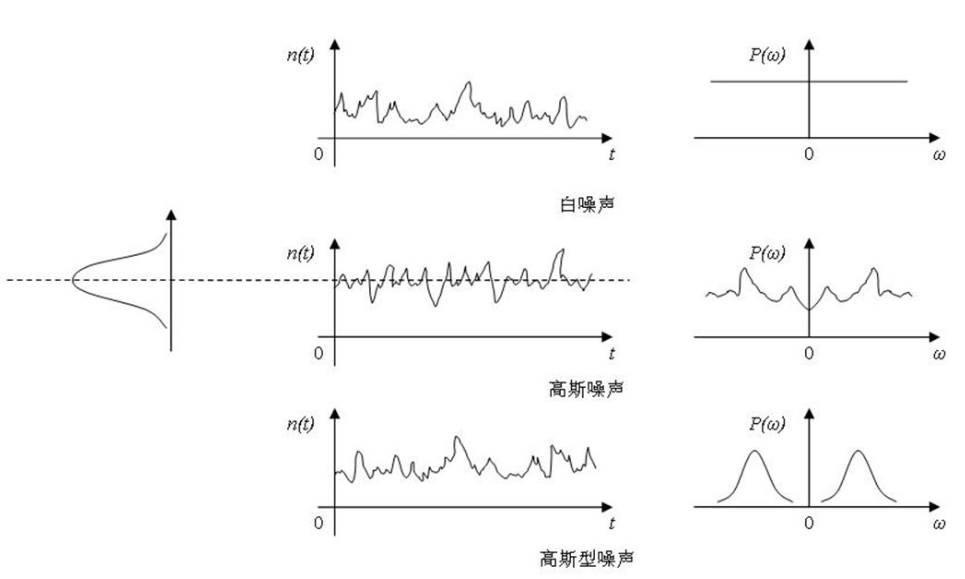
\includegraphics[scale=0.2]{nt}
\end{frame}

\begin{frame}{高斯噪声/白噪声/高斯白噪声(2)}
\url{https://blog.csdn.net/hd19890207/article/details/73498251}
白噪声是指功率谱在整个频域内为常数的噪声,其傅氏反变换是单位冲击函数的n倍(n取决于功率谱的大小),说明噪声自相关函数在t=0时不为零,其他时刻都为0,自相关性最强。

高斯噪声是一种随机噪声,其幅度的统计规律服从高斯分布。高斯白噪声是幅度统计规律服从高斯分布而功率谱为常数的噪声, 如果在系统通带内功率谱为常数,成为带限白噪声“高斯”与“白”没有直接关系,有时人们还会提出高斯型噪声,这指的是噪声功率谱呈高斯分布函数的形状而已。 
\end{frame}

\begin{frame}{高斯噪声/白噪声/高斯白噪声(3)}
\url{https://blog.csdn.net/z_sweet1996/article/details/79183255}

\textbf{白噪声}

白噪声序列,是指白噪声过程的样本实称,简称白噪声。白噪声是在较宽的频率范围内,各等带宽的频带所含的噪声能量相等的噪声,是一种功率频谱密度为常数的随机信号或随机过程,也就是说,此信号在各个频段上的功率是一样的。

对于一个随机变量$X(t)(t=1,2,3\dots)$,如果是由一个不相关的随机变量的序列构成的,即对于所有$s$不等于$t$,随机变量$X(t)$和$X(s)$的协方差为零,则称其为纯随机过程。对于一个纯随机过程来说,若其期望为0,方差为常数,则称之为白噪声过程。
\end{frame}

\begin{frame}{高斯噪声/白噪声/高斯白噪声(4)}
\url{https://blog.csdn.net/z_sweet1996/article/details/79183255}

\textbf{白噪声}

理想的白噪声具有无限的带宽,因而其能量无限大,这是不可能实际存在的,所以,我们把有限带宽内的平整讯号视为白噪声,以便我们实际应用当中的分析。一般情况下,若一个噪声过程所具有的频谱宽度远远大于它所作用系统的带宽,并且在该带宽中其功率谱密度基本为一常数,那么就能够把其作为白噪声来对待。

白噪声的功率密度函数恒定,为:\\
$P_n=\frac{N_0}{2}(-\infty<f<+\infty)$\\
$P_n=N_0(-\infty<f<+\infty)$\\
其中$N_0$为常数
\end{frame}

\begin{frame}{高斯噪声/白噪声/高斯白噪声(5)}
\url{https://blog.csdn.net/z_sweet1996/article/details/79183255}

\textbf{高斯白噪声}

高斯噪声指的是它的概率密度函数服从正态分布的噪声。高斯分布,记为$\mathcal{N}(\mu,\sigma^2)$,其中$\mu$为高斯分布的均值(数学期望),$\sigma^2$为高斯分布的方差,当$\mu=0,\sigma^2=1$时,该分布称为标准正态分布。高斯分布的一维概率密度可表示为:
\[P(x)=\frac{1}{\sqrt{2\pi}\sigma}\exp[-\frac{(x-\mu)^2}{2\sigma^2}] \]
在通信信道中,一般噪声的均值μ=0。那么可以得知当噪声的均值是零的时候,噪声的平均功率等于其方差。

高斯白噪声的高斯指的是概率分布为正态分布,白噪声指的是其二阶矩不相关一阶矩为常数。故把瞬时值的概率分布服从高斯分布,功率谱密度服从均匀分布的噪声称为高斯白噪声。这两个条件是判断高斯白噪声性能的标准。

由于高斯白噪声能够反映实际通信信道中的噪声情况,能够比较真实的反映信道噪声的一些特性,并且可以用具体的数学表达式表示,适合分析、计算系统的抗噪声性能,所以广泛应用于通信系统的理论分析。
\end{frame}

\section{课件公式}

\begin{frame}
$\delta_{jk}=
\begin{cases}
	1, & (j=k)\\
	0, & (j\ne k)
\end{cases}
$, $k=1,2,\dots$
\end{frame}

\begin{frame}
\[\int_{0}^{T}a^2\sin^2(\omega t)dt=\frac{a^2T}{2}, T=2\pi/\omega\]
\[s(t)=\lim\limits_{N\to \infty}\sum_{1}^{N}s_kf_k(t)\]
\begin{align*}
E_s&=\int_{0}^{T}s^2(t)dt\\
&=\int_{0}^{2\pi}(5\sin(t))^2dt\\
&=25\pi
\end{align*}
\end{frame}

\begin{frame}
\begin{align*}
\mu_x(t)&\mathop{=}^{def}E[x(t)]=\int_{-\infty}^{\infty}xp(x;t)dx&\\
E[\int_{0}^{T}x(t)f_k(t)dt]&=\int_{-\infty}^{\infty}\int_{0}^{T}x(t)f_k(t)dtp(x;t)dx\\
&=\int_{0}^{T}\int_{-\infty}^{\infty}x(t)f_k(t)p(x;t)dxdt\\
&=\int_{0}^{T}\left(\int_{-\infty}^{\infty}x(t)p(x;t)dx\right)f_k(t)dt\\
&=\int_{0}^{T}E[x(t)]f_k(t)dt\\
\end{align*}
\end{frame}



